\documentclass[a4paper,10pt]{article}
\usepackage[utf8x]{inputenc}
\usepackage{graphicx}
\usepackage{pgf}
\pgfdeclareimage[height=1cm]{myimage}{p1_q1.png}
\usepackage{listings}

%----------------- CONFIGURAÇÃO PARA OS COMANDOS -----------------------
\lstset
{
  basicstyle = \footnotesize, 		% Tamanho da fonte do código
  %numbers = left, 			% Posição da numeração das linhas
  %numberstyle = \tiny\color{blue}, 	% Estilo da numeração de linhas
  %stepnumber = 1, 			% Numeração das linhas ocorre a cada quantas linhas?
  %numbersep = 10pt, 			% Distância entre a numeração das linhas e o código
  backgroundcolor = \color{white}, 	% Cor de fundo
  showspaces = false, 			% Exibe espaços com um sublinhado
  showstringspaces = false, 		% Sublinha espaços em Strings
  showtabs = false, 			% Exibe tabulação com um sublinhado
  frame = single, 			% Envolve o código com uma moldura, pode ser single ou trBL
  rulecolor = \color{black}, 		% Cor da moldura
  tabsize = 2, 				% Configura tabulação em x espaços
  captionpos = b, 			% Posição do título pode ser t (top) ou b (bottom)
  breaklines = true, 			% Configura quebra de linha automática
  breakatwhitespace= false, 		% Configura quebra de linha
  title = \lstname, 			% Exibe o nome do arquivo incluido
  %caption = \lstname, % Também é possível usar caption no lugar de title
  keywordstyle = \color{blue}, 		% Estilo das palavras chaves
  commentstyle = \color{dkgreen}, 	% Estilo dos Comentários
  stringstyle = \color{mauve}, 		% Estilo de Strings
  escapeinside = {\%*}{*)}, 		% Permite adicionar comandos LaTeX dentro do seu código
  morekeywords     ={*,...} 		% Se quiser adicionar mais palavras-chave
}

%------------------------------------------------------------------------
%------------------------- CAPA -----------------------------------------
%------------------------------------------------------------------------
\title{Projeto Petrolimpa}
  \author{Leonardo Macedo, Rodrigo Siqueira (9868770)}

%------------------------------------------------------------------------
%------------------------- ÍNDICE E DEMAIS ITENS ------------------------
%------------------------------------------------------------------------
\begin{document}
\maketitle
\titlepage
\tableofcontents

%------------------------------------------------------------------------
%------------------------------- Visão geral ----------------------------
%------------------------------------------------------------------------
\newpage
\section{Visão Geral: o problema}

\paragraph{}
Na disciplina de orientação a objetos ministrada no IME pelo professor Fábio
Kon, foi lançado o desafio de modelar um sistema para uma petrolífera na qual
visasse a transparência. Neste sentido, o seguinte enunciado foi fornecido:

\paragraph{}
\emph{"Você foi contratado por uma grande empresa petrolífera para projetar um
sistema de combate à corrupção interna.}

\paragraph{}
\emph{O sistema deve executar de forma distribuída nos 5 escritórios da empresa
espalhados pelo país, coletando dados dos 1.000 postos de gasolina, 20
plataformas de petróleo, 30 centros de distribuição de combustível e 10
refinarias. Não há um único ponto de centralização do sistema, os 5 escritórios
são independentes.}

\paragraph{}
\emph{O sistema utilizará uma motor de inferência (utilizando técnicas de
mineração de dados e IA para localizar suspeitas de fraudes que serão postadas
publicamente, diariamente no web site da empresa).}

\paragraph{}
\emph{Cada compra da empresa (que acontecem a uma taxa de milhares por dia,
espalhadas pelo país) pode ser com licitação ou dispensa de licitação. Além
disso, cada compra pode ser de serviços, de equipamentos permanentes ou de
insumos. Finalmente, cada compra pode ser via importação ou no mercado interno.
Para cada tipo diferente de compra, os algoritmos de detecção de fraudes são
diferentes, i.e., personalizados para cada caso. Além disso, há algoritmos
próprios para detectar fraudes analisando-se a totalização dos gastos de cada
unidade (posto, plataforma, centro de distribuição ou refinaria).}

\paragraph{}
\emph{Cada compra deve ser analisada por exatamente 3 escritórios diferentes.}

\paragraph{}
\emph{Você foi contratado por uma grande empresa petrolífera para projetar um
sistema de combate à corrupção interna.}

\paragraph{}
\emph{O sistema deve executar de forma distribuída nos"}

\paragraph{}
Com base no enunciado fornecido, realizamos uma análise em cada um dos pontos
para realizar a modelagem do sistema. Como nem todas as informações foram
dadas, optamos em certos casos em inferir informações do texto com base em
pesquisas específicas da área.

\subsection{Príncipais ideias extraídas do texto}

\paragraph{}
Para tornar mais direta a descrição, segue em tópicos os princípais pontos
tirados do texto:

\begin{enumerate}
  \item Existem 5 escritórios da empresa em locais diferentes;
  \item A coleta de dados acontece das seguintes fontes:
    \begin{itemize}
      \item 1000 postos de gasolina;
      \item 20 plataformas de petróleo;
      \item 30 centros de distribuição;
      \item 10 refinarias.
    \end{itemize}
  \item Os 5 escritórios devem ser independentes;
  \item O sistema utilizará um motor de inferência para minerar dados e aplicar
        algoritmos de IA;
  \item O sistema posta diariamente no site da empresa qualquer suspeita de
        fraude;
  \item As compras são subdividas em diferentes categorias:
      \begin{itemize}
         \item Forma da compra: licitação ou dispensa de licitação;
         \item Tipo da compra: serviços, de equipamentos permanentes ou de
               insumos;
         \item Local da compra: importação ou no mercado interno.
      \end{itemize}
   \item Para cada tipo de compra, algoritmos diferentes de detecção de fraude
      podem ser usados;
   \item Cada compra é analisada por 3 escritórios diferentes.
\end{enumerate}

\paragraph{}
Em vista dos requisitos levantados, optamos por 3 diagramas UML:
\begin{enumerate}
  \item \textbf{Diagrama de Caso de Uso}: Escolhemos esse diagrama, pois
        acreditamos que ele ajuda a ter uma visão maior do sistema e a entender
        os possíveis pacotes necessários;
  \item \textbf{Diagrama de classes}: Este da uma visão mais detalhada de como
        implementar a relação entre os diferentes componentes do sistema;
  \item \textbf{Diagrama de implantação}: O sistema em questão possui algumas
        características muito específicas sobre a forma como ele é distribuído
        por isto tal diagrama é extremamente informativo para esté contexto.
\end{enumerate}

\newpage
%------------------------------------------------------------------------
%---------------- Diagrama de caso de uso -------------------------------
%------------------------------------------------------------------------
\section{Diagrama de Caso de Uso}

\paragraph{}
Veja a Figura \ref{uc} com a modelagem do diagrama de caso de uso do sistema
petrolimpa.

\begin{figure}[ht]
  \centering
  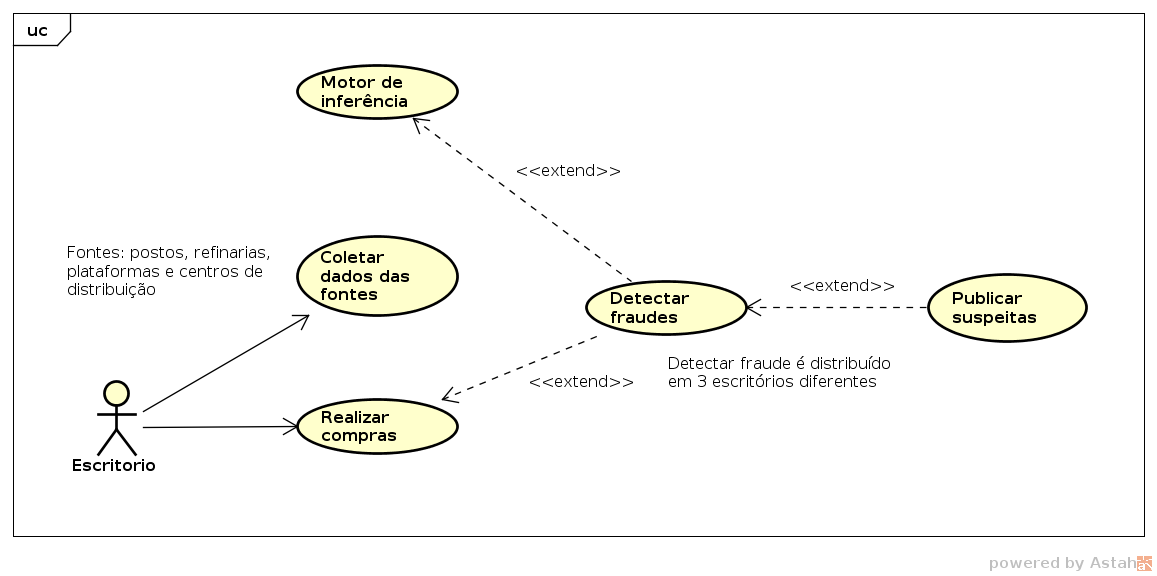
\includegraphics[width=1\textwidth, keepaspectratio=true]{images/uc.png}
  \caption {Diagrama de caso de uso}
  \label {uc}
\end{figure}

Segue a descrição em de cada um dos casos de uso e as suas descrições:

\begin{itemize}
  \item Realizar compras: este caso de uso descreve o procedimento de compras.
        Repare que da sessão anterior, descrevemos as diferentes
        caracteristicas da compra. Está constitui uma parte importante do
        sistema e relaciona-se com outros módulos;
  \item Coletar dados da fonte: Conforme enunciado, o sistema possuí diferentes
        sistemas que fornecem informações de compras e outros. Neste sentido
        este caso de uso visa descrever a forma como estes dados são coletados
        e minerados;
  \item Motor de inferência: O motor de inferência possui os algoritmos de
        mineração e ele é parte do módulo de detecção de fraudes;
  \item Detectar fraudes: Neste módulo é possível encontrar uma enorme
        variedade de algoritmos responsáveis por detectar fraudes;
  \item Publicar suspeitas: Constantemente é preciso realizar a públicação no
        website da empresa com as análises dos dados.
\end{itemize}

%------------------------------------------------------------------------ 
%--------------- Diagrama de classes ------------------------------------
%------------------------------------------------------------------------
\newpage
\section{Diagrama de Classes}

\paragraph{}
O projeto de classes do projeto foi pensando, deixando espaços para a expansão
do mesmo com o menor impacto possível. Em outras palavras, identificamos
potências pontos de alterações no sistema e isolamos eles. Para isto, aplicamos
várias técnicas de OO e a utilização de alguns padrões de projetos. Veja a
Figura \ref{dc} contendo todo o diagrama de classes do projeto (Recomendamos
dar "zoom" no pdf para visualizar com mais detalhes).

\begin{figure}[ht]
  \centering
  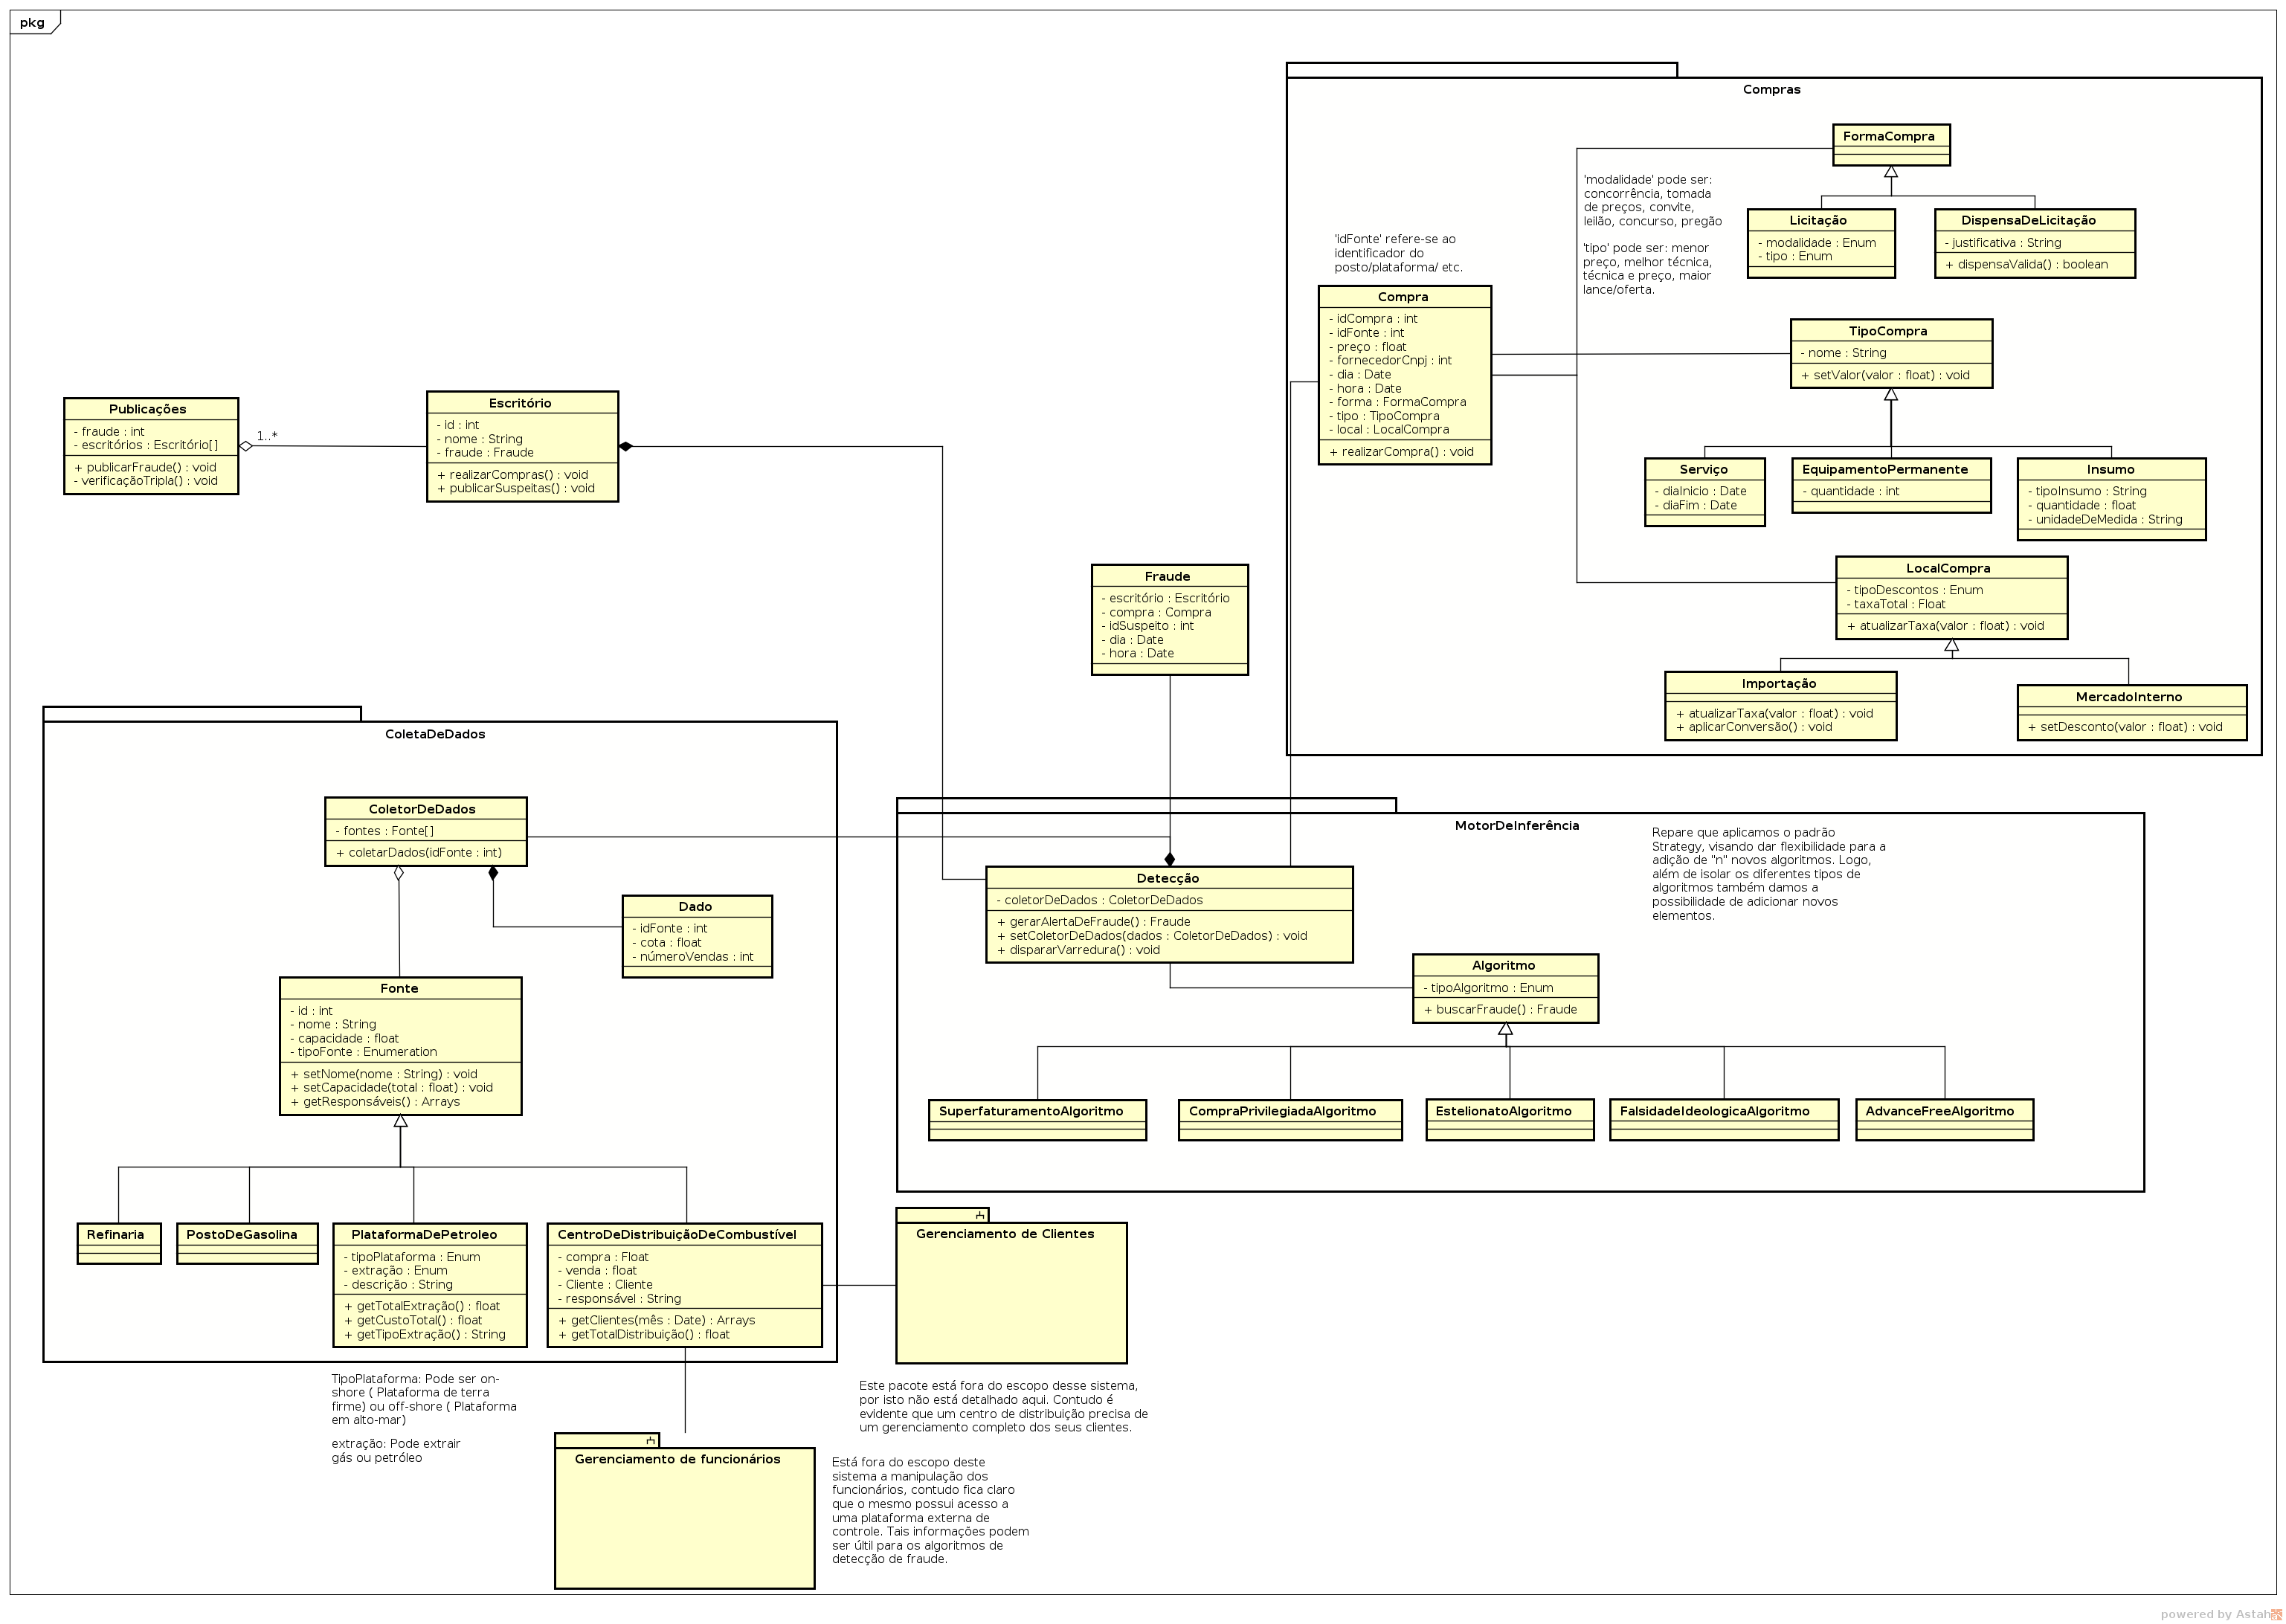
\includegraphics[width=1.3\textwidth, keepaspectratio=true]{images/classes.png}
  \caption {Diagrama de classes completo}
  \label {dc}
\end{figure}

\paragraph{}
Para facilitar a compreensão, explicamos de forma geral cada modulo do
diagrama. Começamos pelo módulo de coleta de dados, responsável por realizar
a aquisição de dados das diferentes fontes do sistema. Veja a Figura
\ref{coleta} e note que os diferente tipos de fontes estão modelados neles e
cada um fornece uma gama diferente de dados. Note que o sistema foi
flexibilizado por meio de uma interface comum que permite a adição de novas
fontes simplesmente extendendo a classe mais abstrata. Por fim, é possível
notar um módulo mais externo chamado ColetorDeDados que visa juntar as diversas
informações.

\begin{figure}[ht]
  \centering
  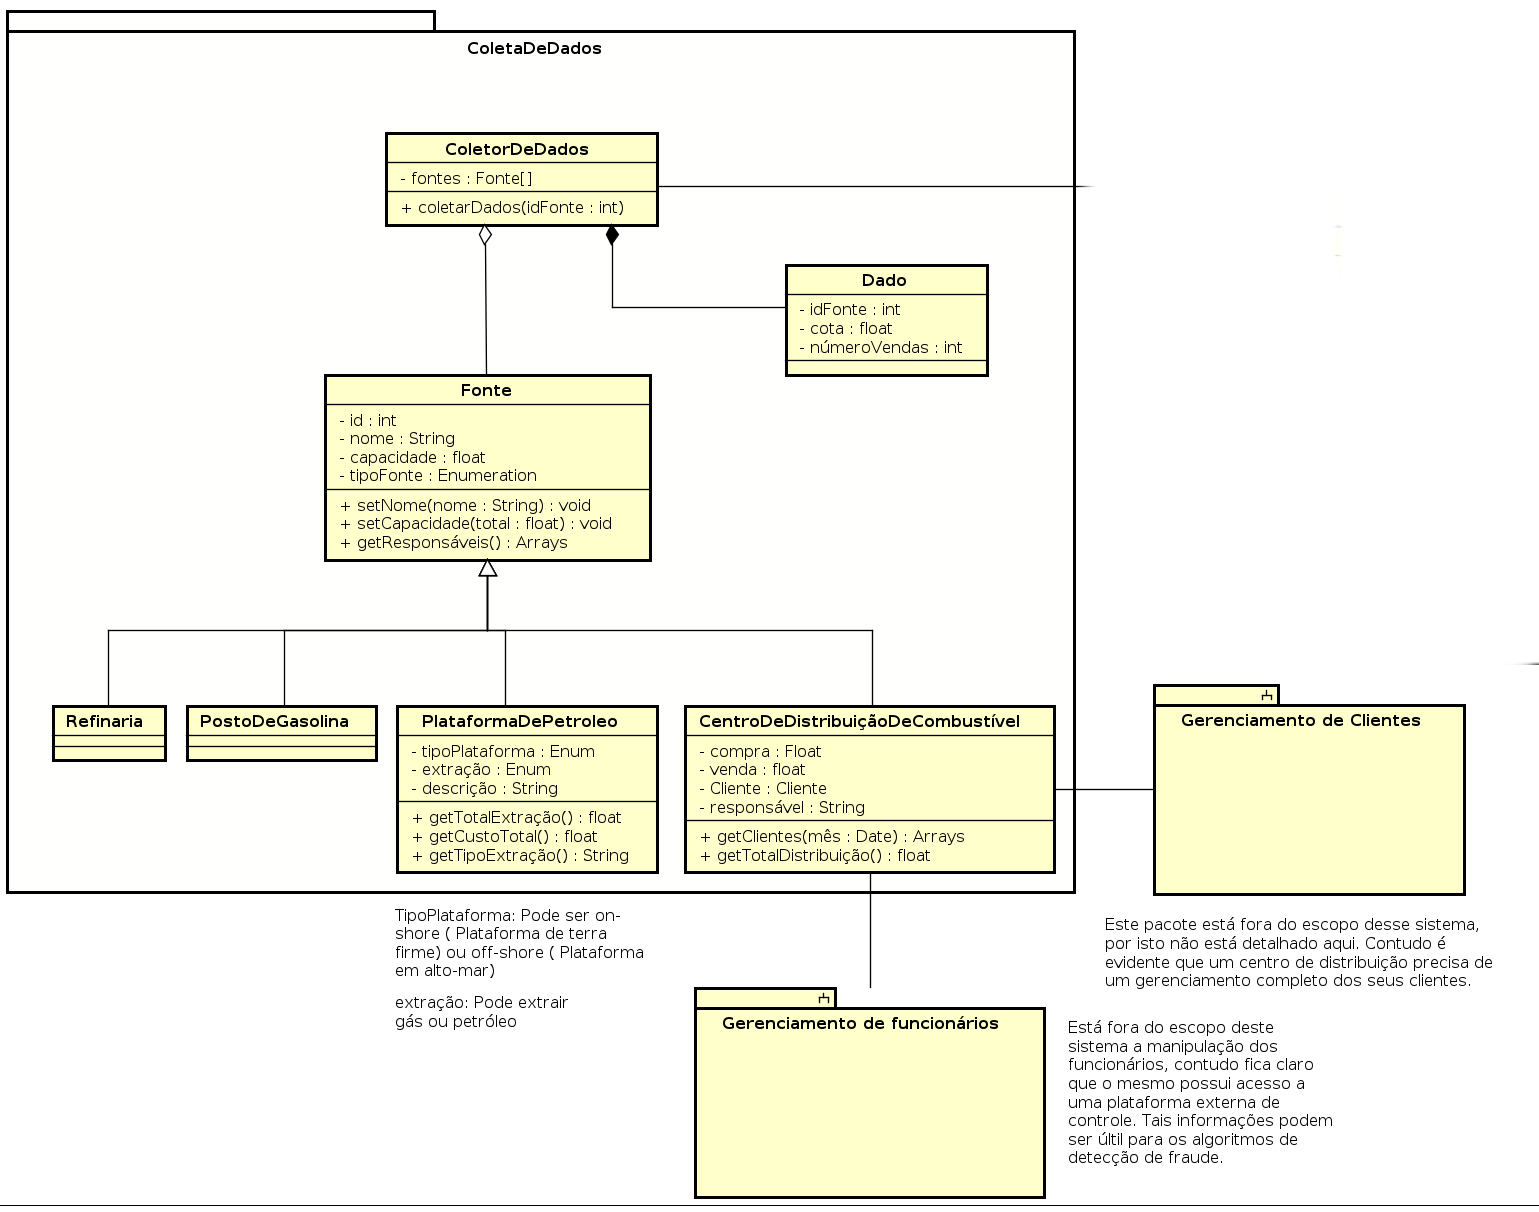
\includegraphics[width=1\textwidth, keepaspectratio=true]{images/coleta.png}
  \caption {Módulo de coleta de dados}
  \label {coleta}
\end{figure}

\paragraph{}
Outro importante módulo do sistema é o motor de inferência, onde é nele que os
dados coletados são passados e os algoritmos de detecção de fraude são
executados. Note que a quantidade de algoritmos possíveis são vastos, dados os
diferentes tipos de fraudes e algoritmos. Veja a Figura \ref{motor} mostrando
como este módulo foi planejado. Repare que aplicamos um padrão de projeto
conhecido como \emph{strategy}, pois notamos que diferentes algoritmos podem
ser inseridos a qualquer momento.

\begin{figure}[ht]
  \centering
  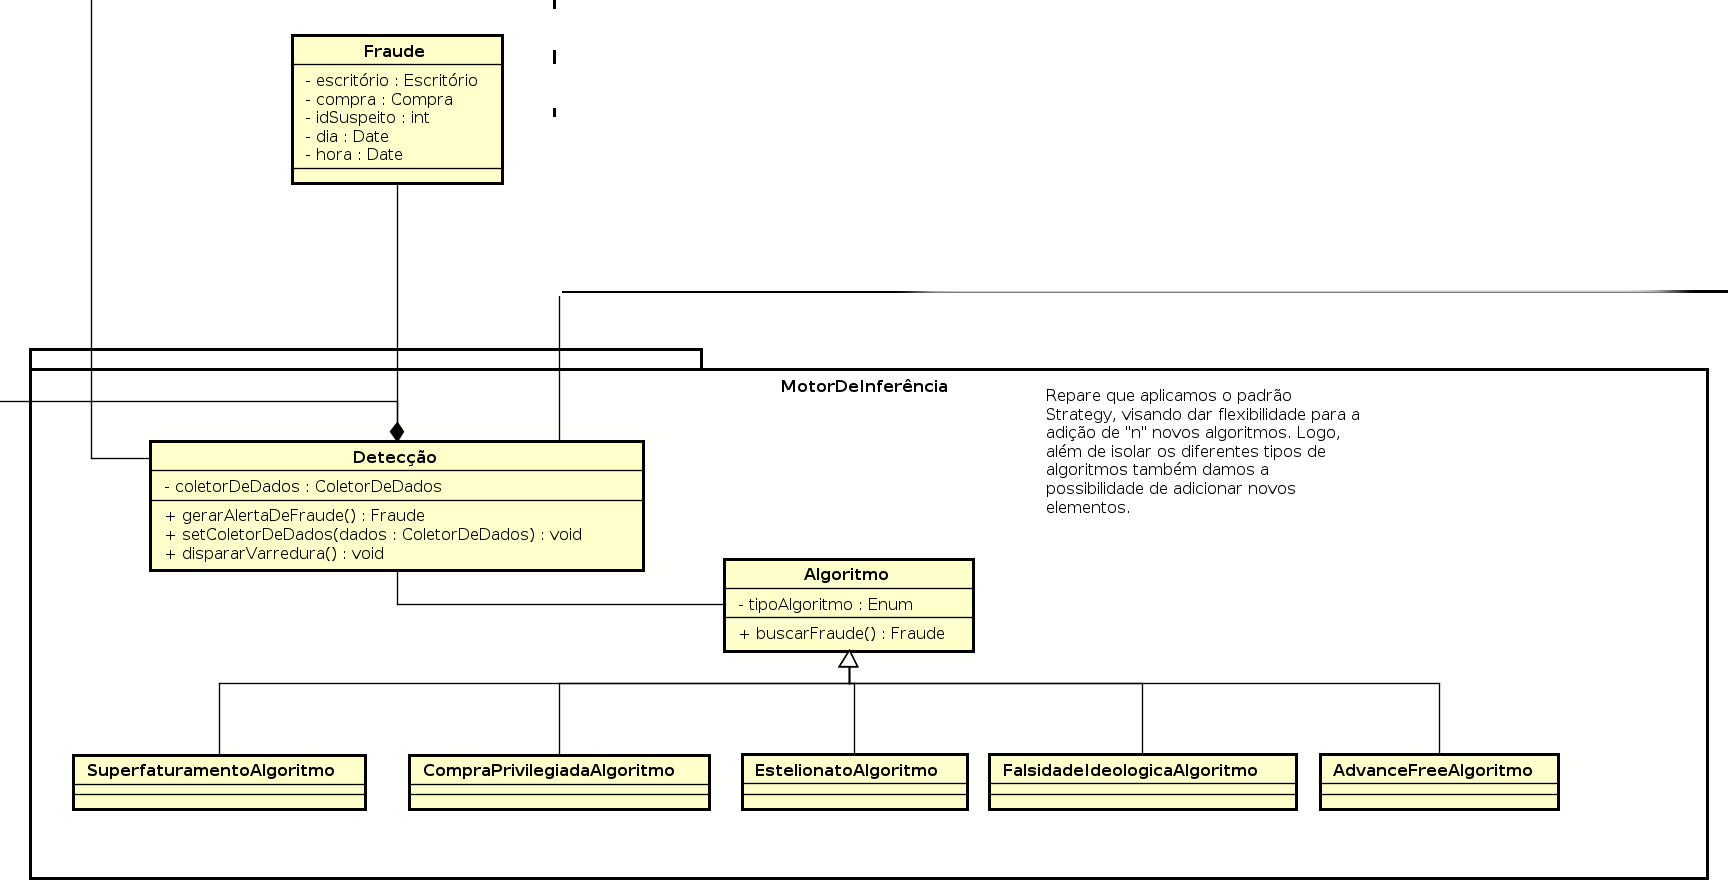
\includegraphics[width=1\textwidth, keepaspectratio=true]{images/motor.png}
  \caption {Módulo do motor de inferência}
  \label {motor}
\end{figure}

\paragraph{}
Um importante módulo do sistema é o de compras, visto que esté pode ser um dos
pontos onde pode ocorrer fraudes. Com base nas informações dada no enunciado e
em uma pesquisa feita sobre os termos utilizados, realizamos a modelagem
apresentadada na Figura \ref{compras}. Note que mais uma vez aplicamos o padrão
\emph{strategy}, mas de uma forma mais ampla com diferentes interfaces para os
manipular os diferentes aspectos de compras.

\begin{figure}[ht]
  \centering
  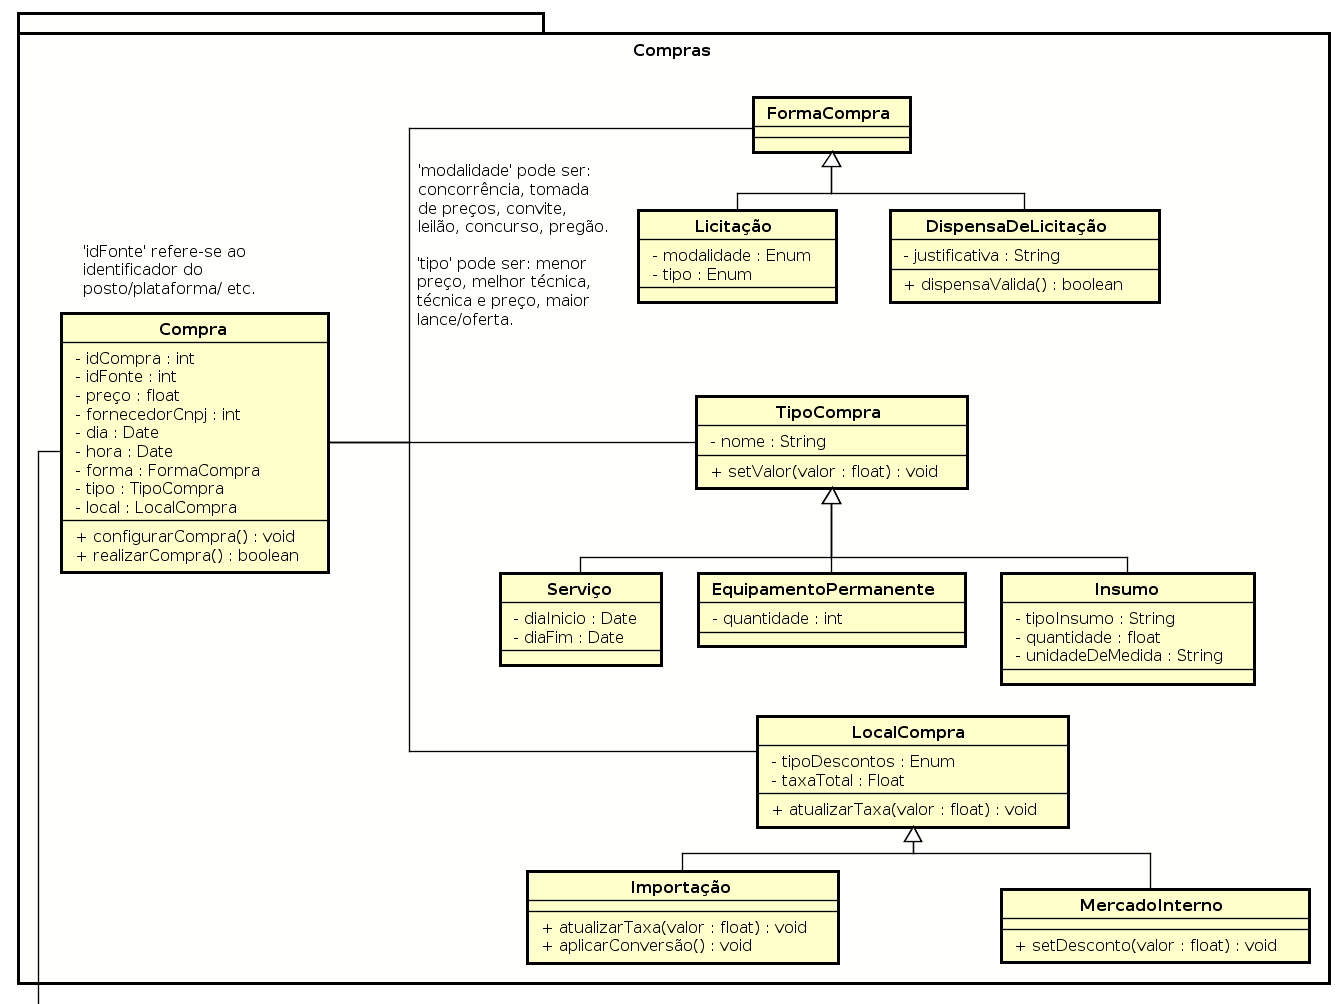
\includegraphics[width=1\textwidth, keepaspectratio=true]{images/compras.png}
  \caption {Módulo de compras}
  \label {compras}
\end{figure}

\newpage
\section{Diagrama de implantação}

\begin{figure}[ht]
  \centering
  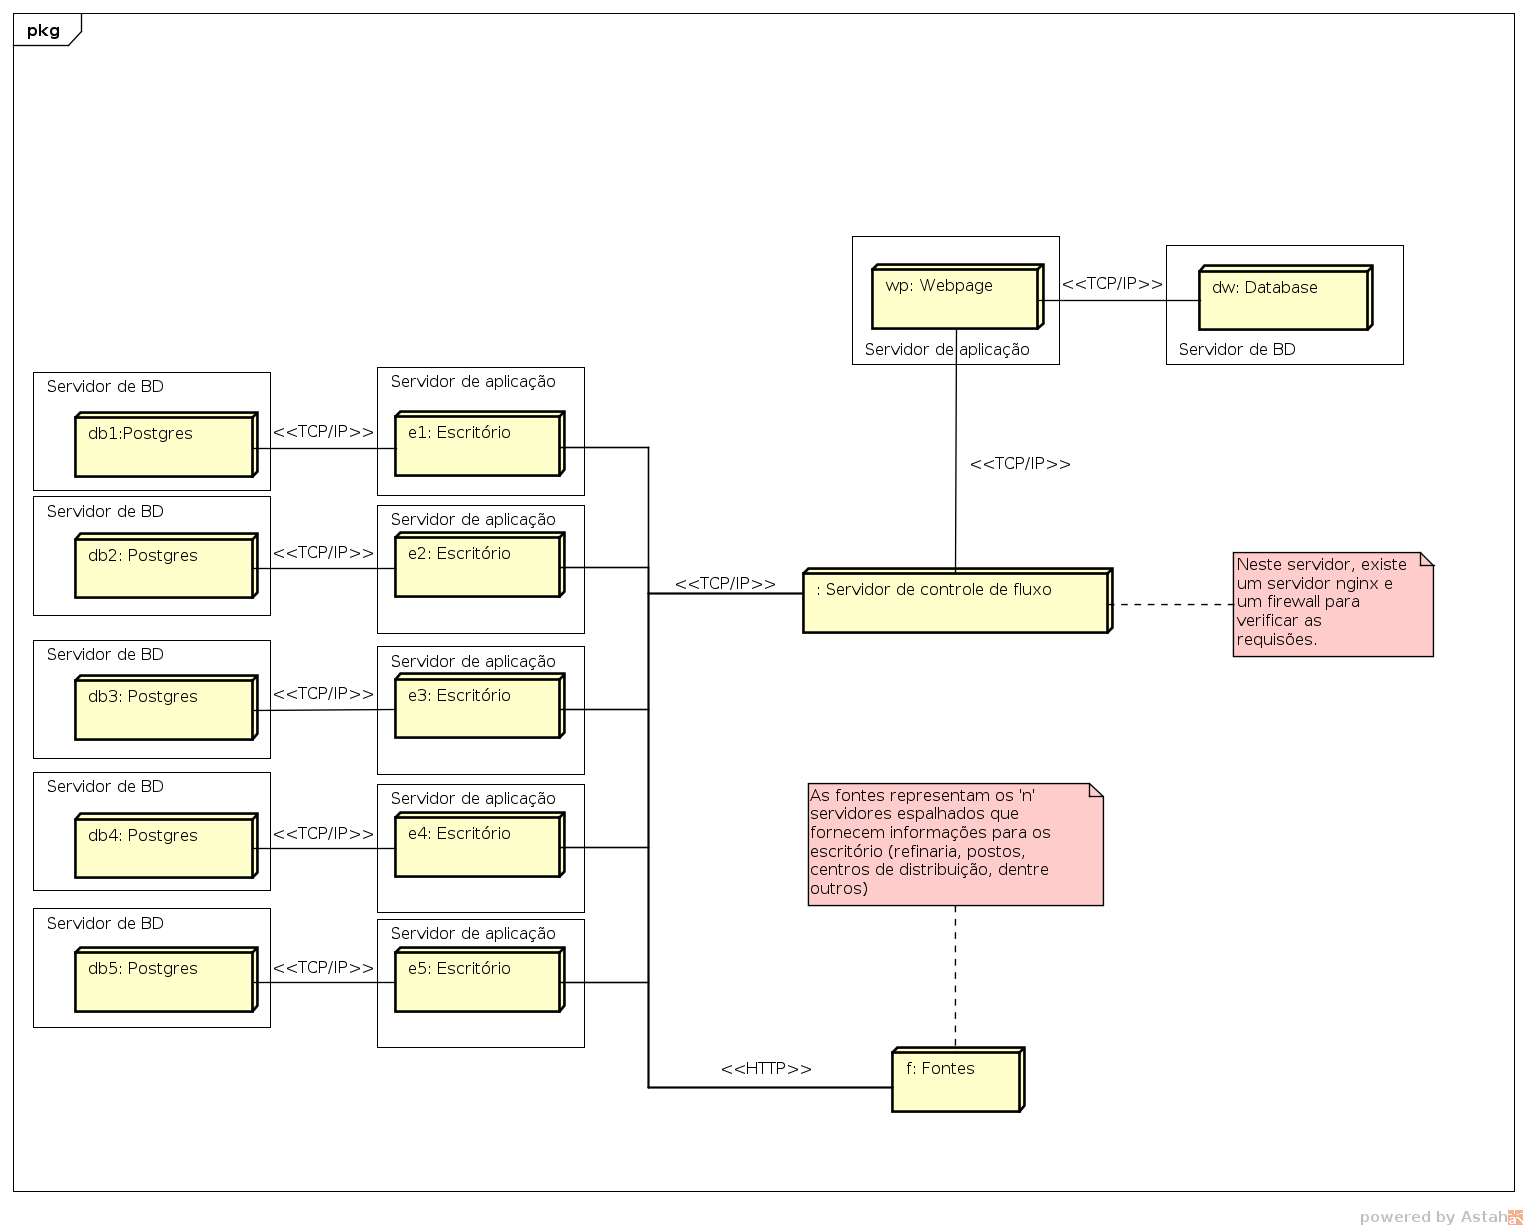
\includegraphics[width=1\textwidth, keepaspectratio=true]{images/DiagramaDeImplantacao.png}
  \caption {Diagrama de implantação}
  \label {di}
\end{figure}

\paragraph{}
O último diagrama utilizado foi o de implantação. Veja a Figura \ref{di} com o
diagrama de implantação adotado para o projeto. Note que os 5 escritórios foram
modelados de maneira similar (um servidor de aplicação e um servidos de banco
de dados), mas todos separados ilustrado a natureza distribuida do sistema.
O sistema web que pública as possíveis fraudes foi colocado a parte conectado
aos 5 escritórios, por uma questão de controle foi adicionado uma camada extra
que recebe as requisições, trata elas e só em seguida passa para a aplicação
web. Por fim as diferentes fontes foram conectadas via HTTP, uma vez que elas
estão localizadas em diferentes pontos e podem possuir diversas implementações
diferentes por isto a utilização do protocolo em questão facilita a
distribuição do sitema.

\end{document}
